\newpage
\section{Diskussion}
	\label{sec:diskussion}
	Die Durchf"uhrung dieses Versuches war vergleichsweise einfach, da die Proben vom Versuchsleiter getauscht wurden.
	Lediglich die Zeitmessung musste eigenst"andig durch\-ge\-f"uhrt werden.
	Fehlerquellen durch den Versuchsaufbau konnten somit gering gehalten werden.

	Die Messwerte waren dementsprechend gut.
	Die Abweichungen von Literaturwerten \cite{halbwertszeiten} betrugen f"ur Indium $\SI{13}{\percent}$.
	Unter Ber"ucksichtigung der Fehler erhielt man $\SI{7}{\percent}$. 
	F"ur Rhodium-104 betrug sie $\SI{2}{\percent}$ und f"ur Rhodium-104i $\SI{3}{\percent}$.

	Bei der Messreihe f"ur Indium ist ein Fehler durch die relativ wenigen Messwerte zu erkl"aren.
	Tr"agt man die Werte nicht-logarithmisch auf, erkennt man nur einen kleinen Teil der Zerfallskurve.

	Die Werte f"ur Rhodium sind relativ gut.

	\begin{figure}[!h]
		\centering
		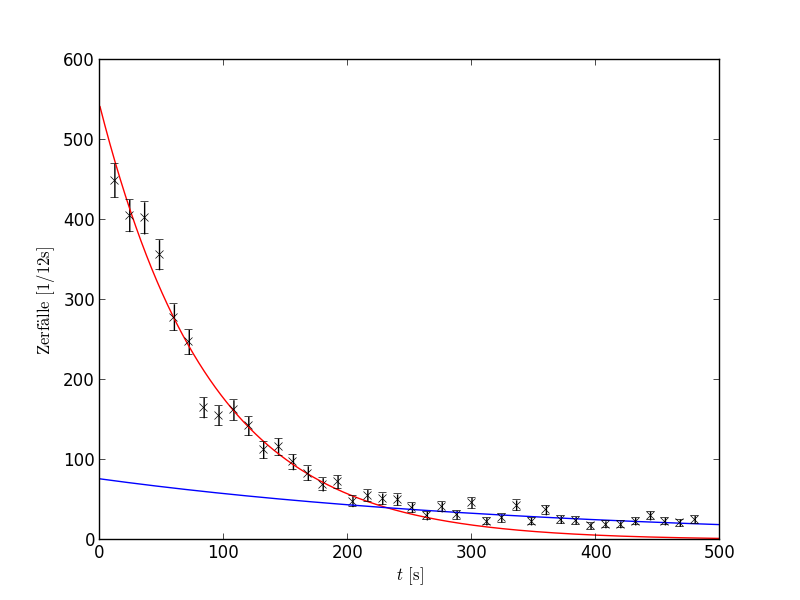
\includegraphics[width = 13cm]{img/graph_indium.png}
		\caption{Zerfallskurve von Indium: Nur ein kleiner Teil des Verlaufs wurde durch die Messwerte sichtbar}
		\label{fig:indium_orig}
	\end{figure}

	\enlargethispage{2cm}

\begin{thebibliography}{9}
	\bibitem{anleitung} Physikalisches Anf"angerpraktikum der TU Dortmund: Versuch Nr. 702 - Aktivierung mit Neutronen. Stand: November 2012.

	\bibitem{halbwertszeiten}  National Nuclear Data Center, Brookhaven National Laboratory. \url{http://www.nndc.bnl.gov/chart/}. Stand: 28.11.12
\end{thebibliography}